% !TeX encoding = UTF-8
% !TeX program = pdfLaTeX
% !TeX root = matlab-exercises-emaip.tex
% !TeX spellcheck = en_GB
\section{Plotting}

To plot eg. the sine function in matlab, the following code
can be used:
\begin{lstlisting}
% Open figure 1
figure(1);

% Clear the content of figure one (this only have an effect 
% if figure 1 already contained previously plotted material)
clf;

% Generate a list of x values, for which the function should be 
% plotted.
x = linspace(-2, 7);

% Plot the function
plot(x, sin(x));
\end{lstlisting}

\subsection{Plotting multiple things in the same plot}

By default matlab will overwrite the content of a figure
when a new plot command is issued.
So for instance if you want to plot both the sine and the cosine 
function in the same plot, this approach would fail, as only the 
cosine function will be present in the generated plot.

\begin{lstlisting}
figure(1);
clf; 
x = linspace(-2, 7);
plot(x, sin(x));
plot(x, cos(x));
\end{lstlisting}

To plot multiple things in the same plot, matlab should be told
to keep using the same ``paper'' that the plot is drawn upon.
This is achieved by the \verb!hold on! command.
After a \verb!hold on! command is issued, matlab will not erase 
the content of a plot but will add new material to the plot.

\begin{lstlisting}
figure(1);
clf; 
x = linspace(-2, 7);
plot(x, sin(x));
hold on;
plot(x, cos(x));
\end{lstlisting}

The plot can be taken out of the \verb!hold on! state, by the 
command \verb!hold off! or by clearing the figure using the 
command \verb!clf!.


\subsection{Plotting constant values}

To visualize an equation like $0.5 = \sin(x)$, 
both sides of the equation can be plotted.
Solutions to the equation is then found 
where the two plotted lines intersect.

However the direct approach for plotting the two sides of the
equations does not work.
The code below will only plot the right hand side of the equation.
\begin{lstlisting}
figure(1);
clf; 
hold on;
x = linspace(-2, 7);
plot(x, sin(x));
plot(x, 0.5);
\end{lstlisting}
The issue is the line
\begin{lstlisting}
plot(x, 0.5);
\end{lstlisting}
As the number of x coordinates and y coordinates does not match, 
Matlab is not able to plot the function with the constant value.
The solution is to modify the code as follows:
\begin{lstlisting}
plot(x, 0.5+0*x);
\end{lstlisting}
The idea is that by adding \verb!0*x! to the constant value, 
it is changed from a single value, to a list of values with the same
number of elements as the vector \verb!x!.



\subsection{Locate points in a plot}
\label{ssecLocatePointsInAPlot}

Sometimes it is practical to get a precise location 
of something that is seen in a plot.
If you for instance want to find a graphical solution to 
the equation
\begin{align*}
e^{-x^2} = 0.2x + 0.5
\end{align*}
the two sides of the equation can be plotted
in the same figure with the commands.
\begin{lstlisting}
figure(1);
clf; 
x = linspace(-3, 3);
fh_left = @(x) exp(-x.^2);
fh_right = @(x) 0.2*x + 0.5;
plot(x, fh_left(x));
hold on;
plot(x, fh_right(x));
\end{lstlisting}
When the figure is shown, you can now issue the command
\begin{lstlisting}
solutions = ginput(3)
\end{lstlisting}
which will put the figure in focus and show a cross hair 
with which you can click on the three locations where the 
two curves intersect.
The $x$,  $y$ coordinates of the locations that were clicked is 
then saved in the variable \verb!solutions!.


\subsection{Adding information to plots}
\label{ssecAddingInformationToPlots}

It is often beneficial to add some text to plots, 
that can describe what is visualized and what are on the 
axes. 
This can be achieved using the commands \verb!title!, 
\verb!xlabel! and \verb!ylabel! as shown here:
\begin{lstlisting}
title("Harmonic oscillations")
xlabel("Time [s]")
ylabel("Offset")
\end{lstlisting}

If you need to add mathematical expression it is possible 
for matlab to visualise latex expressions.
To do this specify that the latex interpreter is used when 
formatting text as shown here:
\begin{lstlisting}
title("Harmonic oscillations $a^b$", 'interpreter', 'latex')
xlabel("Time $t$ [s]", 'interpreter', 'latex')
ylabel("Offset $\sin(t)$", 'interpreter', 'latex')
\end{lstlisting}


\subsection{Specifying plot limits}

For some plots it is only of interest to show a specific 
part of the coordinate system.
To choose which part to include in a plot, use the 
\verb!xlim! and \verb!ylim! commands.


\subsection{Adding text annotations to a plot}

Text elements can be placed in the plot area
using the \verb!text! command.
The command requires three arguments, the location of the 
text specified as $x$ and $y$ coordinates and the 
text to insert.
It is also possible to insert mathematical expressions
using the \verb!text! command as described in 
\ref{ssecAddingInformationToPlots}.


\subsection{Multiple plots in each figure}

On information about how to add multiple
plots to a single figure, see section 
\ref{ssecMultiplePlotsInOne}.


\subsection{Exporting a plot to an image}

When a plot has been generated in matlab, 
it is often practical to export the plot as an image.
This makes it possible to include the plot in a 
report or similar document.
To export the current plot as a png image, the command
\verb!print! can be used as follows:
\begin{lstlisting}
print('subplot_example_1.png', '-dpng', '-r300');
\end{lstlisting}
In the example the print command takes a filename as input 
as well two options specifying the fileformat (png) 
and resolution of the exported image.


\subsection{Aspect ratio}

\begin{wrapfigure}{r}{6cm}
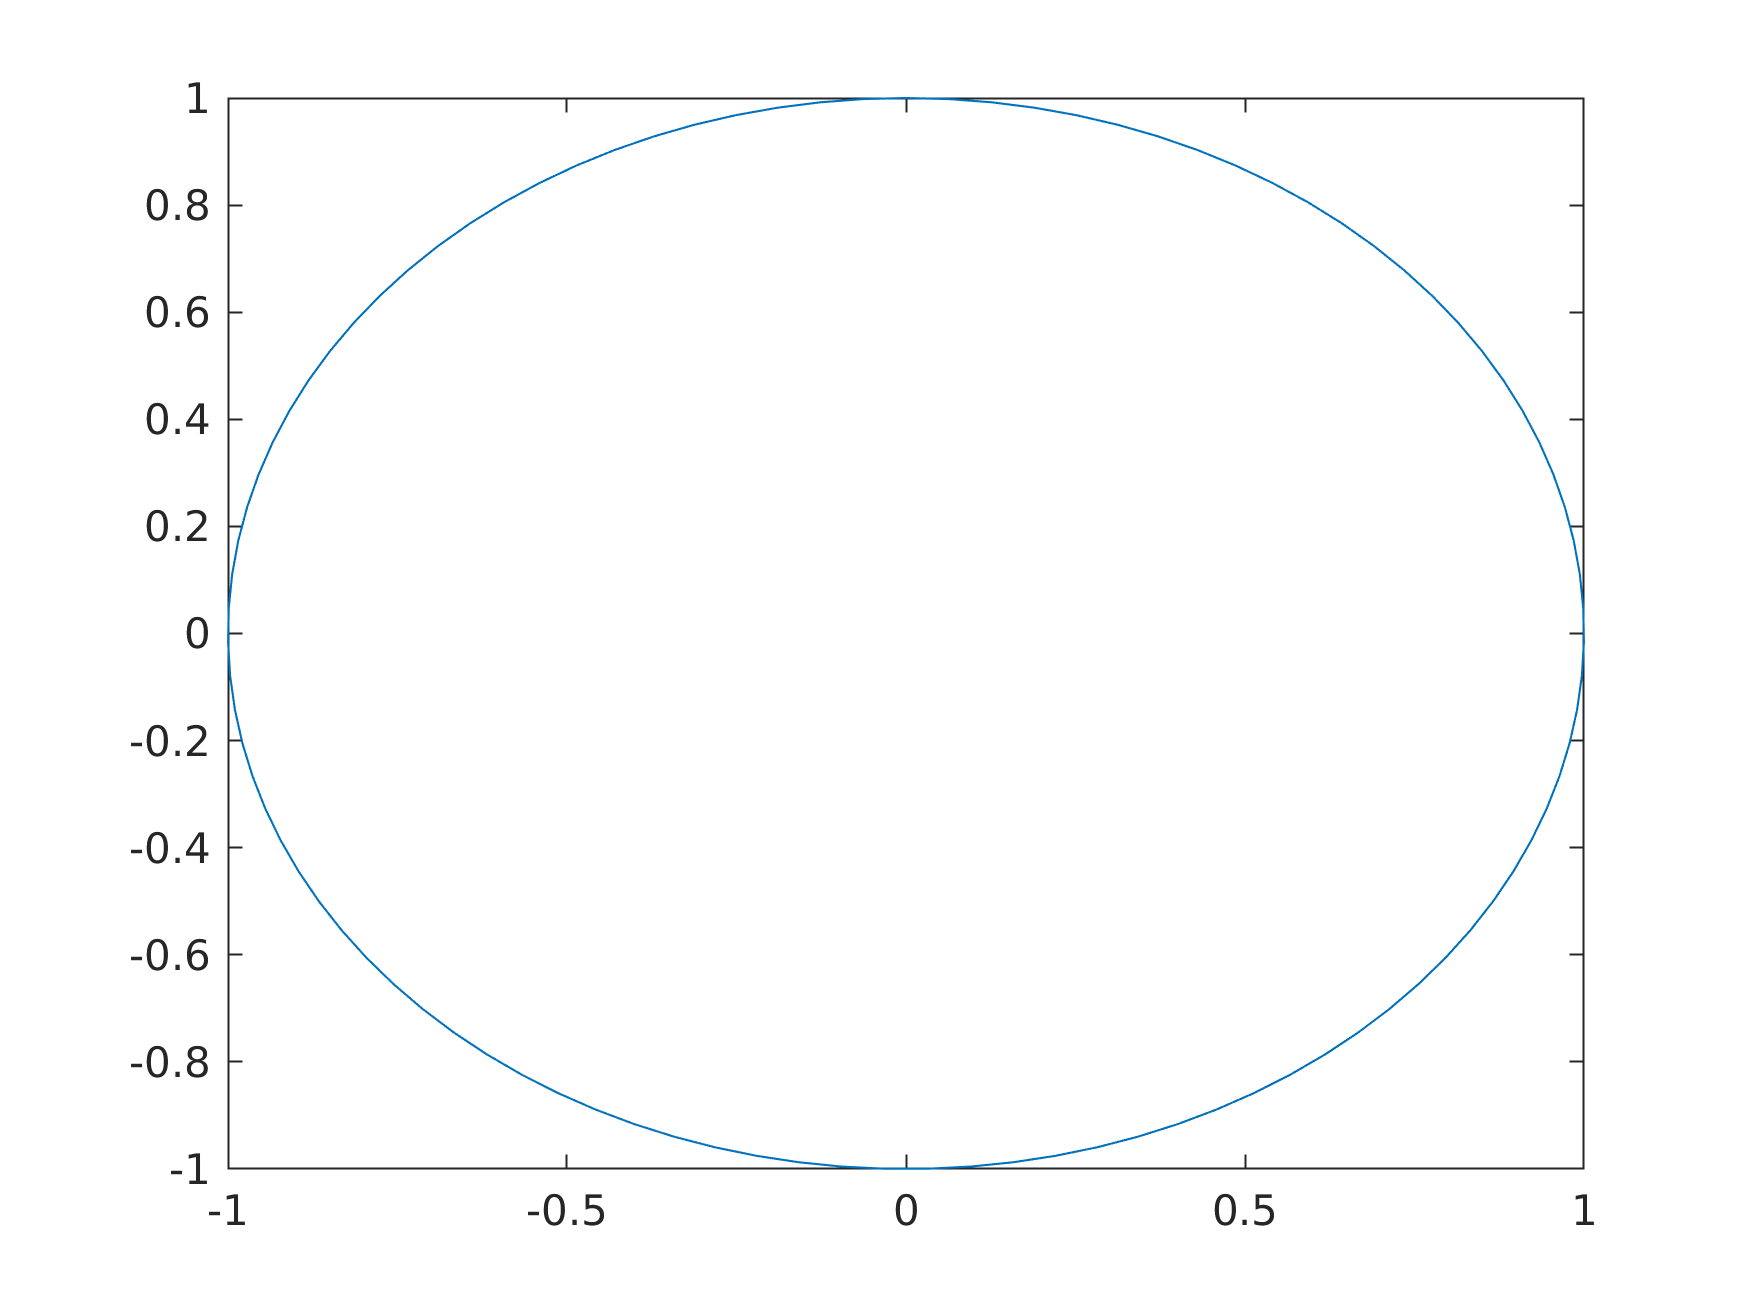
\includegraphics[width=6cm]{pic/plotting/aspect_ratio_free.png}
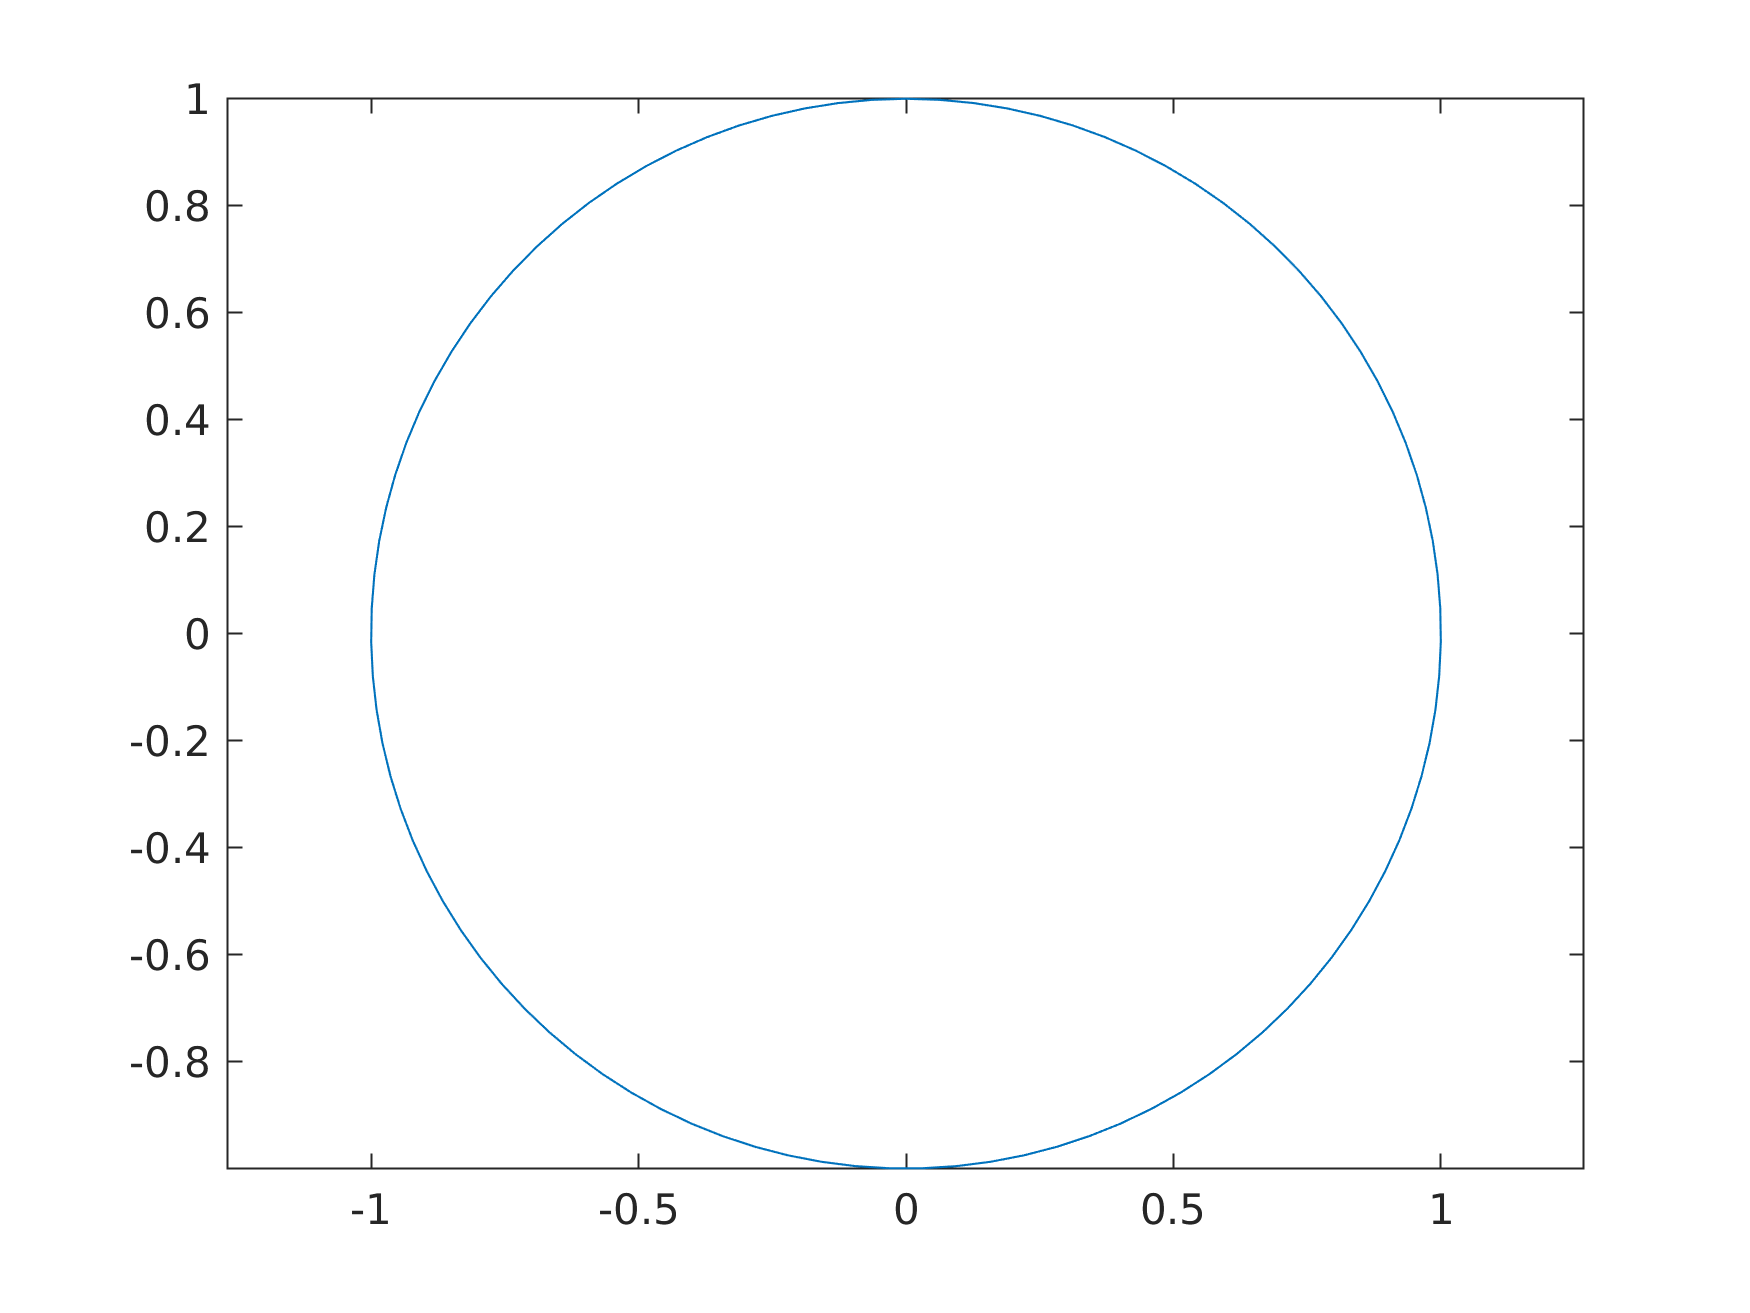
\includegraphics[width=6cm]{pic/plotting/aspect_ratio_equal.png}
\end{wrapfigure}
When plotting coordinates (either real world coordinates in meters
or coordinates in the complex plane), it is good practice to 
ensure that the scaling of the $x$-axis and the $y$-axis is equal.
This makes circles appear as circles instead of ellipses in the plot.
To enforce that the axes are scaled equally, use the matlab
command \verb!axis equal!, as demonstrated in the code snippet
below.
The effect is shown on the plot to the right.

\begin{lstlisting}
theta = linspace(0, 2*pi);
x = sin(theta);
y = cos(theta);
figure(1);
plot(x, y)
figure(2);
plot(x, y);
axis equal;
\end{lstlisting}




 